\chapter{\MakeUppercase{Реализация веб-интерфейса}}
% \label{ch:tab}
%     Наконец, разберемся с таблицами. В принципе, \LaTeX{} позволяет делать большие и сложные таблицы, но вручную обычно их не пишут; для этого используют разные сайты типа \href{https://www.tablesgenerator.com/}{типа такого}. По ГОСТ заморачиваться с таблицами особо не надо, главное чтобы правильно были заданы подписи, работала нумерация и ссылки. Все необходимые стилевые условия уже зашиты в данный шаблон. Помните, что в конце заголовка таблицы, как и в конце подписи к рисунку, точка не ставится! Воспользовавишись сайтом по данной выше ссылке, можем сделать, например, такую таблицу:
% \begin{table}[ht]
% \caption{Вот так выглядит рандомная таблица из Интернета с ценой разных животных, которых можно найти в мире}
% \label{tab:t1}
% \centering
% \begin{tabular}{llr}
% \hline
% Animal    & Description & Price (\$) \\ \hline
% Gnat      & per gram    & 13.65      \\
%           & each        & 0.01       \\
% Gnu       & stuffed     & 92.50      \\
% Emu       & stuffed     & 33.33      \\
% Armadillo & frozen      & 8.99       \\ \hline
% \end{tabular}
% \end{table}

% На эту таблицу, безусловно, можно так же ссылаться. Давайте сошлемся на \hyperref[tab:t1]{Таблицу \ref*{tab:t1}} и на этом, пожалуй, закончим.

В данной главе обозреваются все основные библиотеки, которые были использованы, их интеграция в проект, а также описаны основные архитектурные решения, которые были приняты. Кроме того, демонстрируется текущий функционал разработанного веб-интерфейса.

\section{Основные библиотеки}

Для реализации веб-интерфейса приложения был использован ряд библиотек и инструментов, которые помогли решить конкретные задачи. В данной главе рассмотрены основные библиотеки, использованные для создания функциональности приложения, а также объяснен их выбор и интеграция.

\subsection{Three.js для работы с 3D графикой}
\label{subsec:three}
В проекте возникла необходимость в использовании библиотеки для 3D графики для создания интерактивных сцен и работы с трехмерными объектами. Для работы с 3D графикой в браузере используется WebGL. WebGL – это программная библиотека для JavaScript, которая позволяет создавать 3D графику, функционирующую в браузерах. Данная библиотека основана на архитектуре OpenGL и использует язык программирования шейдеров GLSL, который имеет С-подобный синтаксис. WebGL интересен тем, что код моделируется непосредственно в браузере. Для этого WebGL использует объект canvas, который был введен в HTML5.

Работа с WebGL и с шейдерами в частности — это довольно трудоемкий процесс. В процессе разработки необходимо описать каждую точку, линию, грань и так далее. Чтобы все это визуализировать, необходимо прописать довольно объемный кусок кода. Для повышения скорости разработки была использована библиотека Three.js. Three.js облегчает работу с 3D-графикой, предоставляя интерфейс высокого уровня абстракции, который скрывает техническую сложность использования WebGL.

Three.js был выбран из-за его универсальности и гибкости, что позволяло создавать сложные сцены и анимации. Основным преимуществом использования Three.js является его большое и активное сообщество, которое постоянно поддерживает и развивает библиотеку, обеспечивая большое количество расширений и плагинов, что существенно облегчает разработку \cite{dirksen2014three}. 

Существуют альтернативы, такие как Babylon.js и PlayCanvas, однако Three.js был предпочтительным выбором благодаря своей гибкости и активному сообществу. Кроме того, библиотека AMI.js, которая в проекте используется для работы с DICOM файлами, в ядре также использует Three.js, что обеспечило дополнительную совместимость и упрощение интеграции.

\subsection{Ami.js для работы с DICOM файлами}

Несмотря на широкие возможности, которые предоставляет Three.js, она не имеет встроенной поддержки работы с файлами DICOM напрямую. Это связано с тем, что формат DICOM является стандартом в медицинской практике и имеет свою специфику. Формат DICOM достаточно сложен и обширен, так как охватывает различные типы данных, используемых в медицинской визуализации, такие как КТ, рентген, УЗИ и другие.

Каждый из этих типов данных реализуется через формат DICOM, но они значительно различаются между собой по структуре и содержимому. Внедрение поддержки DICOM в библиотеку Three.js потребовало бы значительных усилий, учитывая разнообразие и сложность формата. Это, вероятно, является основной причиной отсутствия такой поддержки в Three.js, несмотря на её популярность и широкие возможности. Поэтому пришлось использовать сторонние библиотеки.

Среди библиотек для работы с медицинскими изображениями в формате DICOM, AMI.js выделяется тем, что в его основе лежит Three.js, что обеспечивает эффективную работу с трехмерными визуализациями. Варианты альтернатив, такие как Cornerstone с ядром на базе VTK.js, оказались менее подходящими из-за сложности настройки и менее гибкой архитектуры. Однако использование AMI.js не лишено недостатков. Библиотека не обновлялась с 2018 года и изначально была написана на JavaScript, поддерживая версии Three.js до 0.99.0, что является довольно устаревшей версией.

Также стоит отметить, что AMI.js не имеет поддержки TypeScript, что создавало дополнительные трудности в интеграции с современными проектами, использующими строгую типизацию. В ходе проекта пришлось самостоятельно дописывать определения типов для модуля AMI.js. Для написания типизации необходимо было вручную анализировать исходный код библиотеки, что значительно усложняло процесс. В некоторых случаях анализаторы IDE помогали выявить необходимые типы, но зачастую приходилось додумывать их самостоятельно.

В ходе разработки было обнаружено, что при работе со сценой, на которой расположен сагиттальный срез, происходило заметное снижение частоты кадров в секунду до критических уровней, при которых программа фактически зависала. Это особенно заметно проявлялось при высоком разрешении изображаемого среза и большом количестве пикселей.

Этот баг является серьезной проблемой, так как он негативно влияет на производительность приложения, делая его использование затруднительным. Была выдвинута гипотеза о причине этого бага.

Основная гипотеза заключается в том, что проблема связана с отображением воксельной модели. Воксельная модель представляет собой трёхмерный массив данных, где каждый элемент (воксель) содержит информацию о плотности в определенной точке пространства, аналогично тому, как пиксели представляют собой двумерный массив в изображениях.

Для рендеринга воксельных моделей существуют специфичные задачи, связанные с эффективным хранением и доступом к данным. В частности, скорость доступа к данным в различных направлениях в трёхмерном массиве может значительно различаться. Это связано с тем, что расстояние между данными в кэше процессора может варьироваться в зависимости от направления доступа.

Специализированные рендереры для воксельных моделей используют оптимальные методы хранения данных для обеспечения быстрой и эффективной визуализации. Однако, похоже, что в библиотеке AMI.js эти методы либо не были реализованы, либо реализованы недостаточно оптимально, что и приводит к описанным проблемам с производительностью.

На данный момент устранить этот баг не удалось, что ограничивает возможности использования AMI.js для работы с высококачественными медицинскими изображениями. В дальнейшем планируется провести более детальное исследование проблемы и попытаться найти пути ее решения, возможно, с использованием альтернативных библиотек или собственных оптимизаций.

Несмотря на эти минусы и трудности, AMI.js является мощным инструментом для работы с DICOM и предоставляет все необходимые функции для работы с медицинскими изображениями.

\subsection{Dexie.js для хранения данных}

Потребность в личном кабинете доктора возникла из-за необходимости кэшировать данные, загружаемые в приложении. Так как браузерные приложения не имеют прямого доступа к файловой системе, сохранять прогресс работы (например, сегментированные аорты или загруженные снимки) напрямую на компьютер пользователя невозможно. Обновление страницы приводило бы к необходимости заново загружать все данные.

Первоначально предполагалось создать серверную базу данных и серверное приложение для хранения и управления данными. Однако это усложняло бы разработку и требовало создания дополнительных серверных компонентов.

В ходе написания дипломной работы было предложено альтернативное решение: использовать локальную базу данных в браузере для кэширования данных. Индексированная база данных (IndexedDB) позволяет хранить большие объемы данных непосредственно в браузере и предоставляет удобный доступ к ним. Для упрощения работы с IndexedDB была выбрана библиотека Dexie.js.

Dexie.js предоставляет удобный и производительный интерфейс для работы с IndexedDB, позволяя легко сохранять и загружать данные из базы данных. Внедрение Dexie.js позволило перенести кэширование данных с серверной части на клиентскую, что значительно упростило архитектуру приложения и сделало его более независимым от серверных компонентов.

Использование Dexie.js обеспечило следующие преимущества:

\begin{itemize}
    \item упрощение серверной части: Серверная часть приложения не зависит от локальных данных и выполняет только те функции, которые основаны на входных данных от клиента;
    \item безопасность хранения данных: Данные хранятся на компьютере пользователя и могут быть доступны только с того же домена, на котором они были сохранены, что делает их безопасными от несанкционированного доступа;
    \item производительность и масштабируемость: Dexie.js обеспечивает высокую производительность работы с данными и позволяет масштабировать приложение без значительных изменений в его архитектуре.
\end{itemize}

Таким образом, использование библиотеки Dexie.js для работы с локальной базой данных в браузере позволило значительно упростить разработку и улучшить функциональность приложения, обеспечив удобное и безопасное кэширование данных на стороне клиента.

Для хранения информации о пациентах и данных медицинских обследований была разработана следующая схема базы данных\hyperref[fig:bird1]{(Рисунок \ref*{fig:db_scheme})}.

    \begin{figure}[ht]
        \centering
        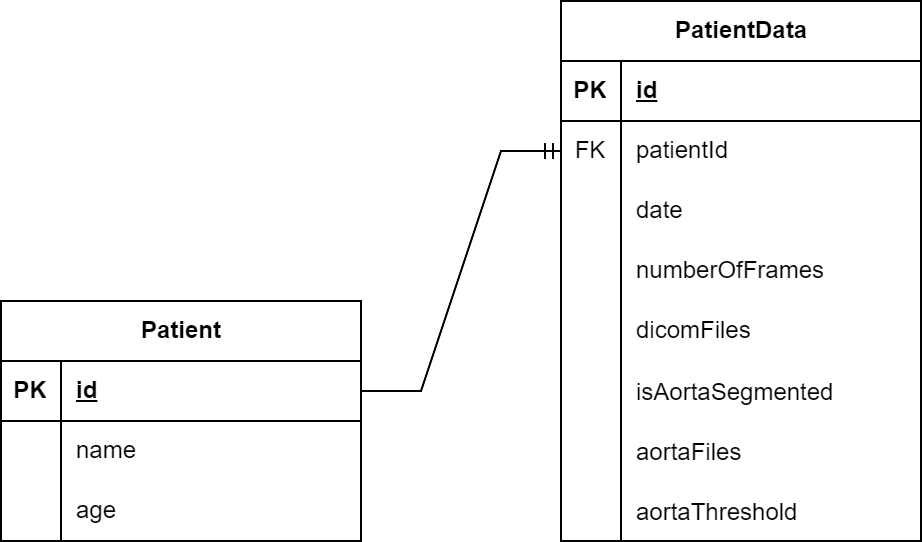
\includegraphics[]{images/chap3/db.drawio.png}
        \caption{Схема базы данных}
        \label{fig:db_scheme}
    \end{figure}
    
В данной схеме база данных состоит из двух таблиц: Patient и PatientData.

\begin{itemize}
    \item таблица Patient содержит основную информацию о пациентах из метаданных;
    \item таблица PatientData предназначена для хранения данных, таких как дата исследования, количество кадров, файлы DICOM, данные сегментации.
\end{itemize}

В будущем планируется модификация данной схемы базы данных для интеграции линий пришиваний и створок клапанов, а также других метаданных пациента при необходимости.

\subsection{Вспомогательные библиотеки для React}

Как было упомянуто в \hyperref[subsec:react]{разделе \ref{subsec:react}}, React сам по себе не является полноценным фреймворком, а скорее библиотекой для создания пользовательских интерфейсов. Для реализации многих ключевых функций требуется использование дополнительных библиотек. В этом разделе мы рассмотрим несколько важных вспомогательных библиотек, которые использовались в проекте.

Для реализации Flux-архитектуры в приложении был выбран Redux. Flux-архитектура помогает управлять состоянием приложения и потоками данных, что особенно важно в больших и сложных приложениях. Redux предоставляет централизованное хранилище для состояния приложения, что позволяет легко управлять состоянием, отслеживать изменения и проводить отладку.

\begin{itemize}
    \item централизованное управление состоянием: Все состояние приложения хранится в одном месте, что упрощает управление и отладку;
    \item предсказуемость: Изменения состояния осуществляются через специальные механизмы, что делает поведение приложения более предсказуемым;
    \item возможность интеграции с различными инструментами: Redux легко интегрируется с различными инструментами для отладки и тестирования.
\end{itemize}

Создание пользовательского интерфейса с нуля может быть трудоемким и времязатратным процессом, особенно когда речь идет о создании стандартных элементов интерфейса, таких как кнопки, списки, панели навигации и т.д. Для упрощения этого процесса была использована библиотека Material-UI.

Material-UI предоставляет набор готовых компонентов, стилизованных в соответствии с принципами Material Design. Это позволяет:

\begin{itemize}
    \item ускорить разработку интерфейса: Использование готовых компонентов экономит время, необходимое на разработку и стилизацию;
    \item обеспечить единый стиль приложения: Все компоненты стилизованы в одном стиле, что делает интерфейс приложения более согласованным и профессиональным;
    \item поддержка и обновления: Material-UI активно поддерживается сообществом разработчиков и регулярно обновляется, что обеспечивает совместимость с новыми версиями React и других инструментов.
\end{itemize}

Эти вспомогательные библиотеки в совокупности с React позволили создать мощный и функциональный веб-интерфейс, который удовлетворяет все текущие потребности проекта и обладает потенциалом для дальнейшего развития и улучшения.

\section{Ключевые моменты реализации}

Далее описаны ключевые моменты, связанные с объединением различных библиотек и инструментов в единую архитектурную систему. Проблема заключалась в необходимости интеграции различных библиотек, таких как React и Three.js, и управления их взаимодействием в рамках единого приложения. Также описаны основные аспекты взаимодействия с серверной частью.

\subsection{Архитектура приложения}

Для создания полноценного веб-приложения необходимо было объединить несколько библиотек, каждая из которых выполняла бы свою специфическую задачу. В нашем случае это React для создания пользовательского интерфейса и Three.js для работы с 3D графикой. Для удобной интеграции Three.js и React существует библиотека React-Three, однако ее использование не было возможно, так как для использования AMI.js нужна версия Three.js 0.99.0, а для React-Three нужна версия Three.js от 0.125.0.

Первоначальной идеей было взять основные подходы из React-Three и реализовать их самостоятельно для нашего приложения, однако возникли трудности.

Парадигма React-Three хорошо подходила для реализации одной сцены или множества независимых сцен, однако у нас все четыре сцены сильно зависели друг от друга, что создавало сложности в реализации такой парадигмы. Работать с изменяемыми объектами в React и Three.js, а также управлять состоянием и взаимодействием между зависимыми сценами, оказалось непросто.

Одной из проблем, с которой пришлось столкнуться при использовании React, является его строгий режим (strict mode). Cтрогий режим важен для разработки, так как помогает отлавливать потенциальные проблемы и побочные эффекты, отрисовывая каждый компонент дважды. Это позволяет React выявить различные ошибки и некорректное поведение на ранних стадиях. Однако использование строгого режима приводило к дублированию некоторых объектов, что создавало проблемы при работе с 3D сценами.

Подход к архитектуре приложения претерпевал значительные изменения на протяжении разработки. В конечном итоге была выбрана парадигма, которая заключалась в инкапсуляции логики работы с 3D сценой и пользовательским интерфейсом. Для их связи был создан удобный API, позволяющий выполнять операции с 3D сценой (например, добавление или удаление элементов) из пользовательского интерфейса.

Основная идея заключалась в инкапсуляции всей логики работы с 3D объектами в специальных классах. Были созданы два ключевых класса: Renderer3D и Renderer2D для работы с трехмерными и двухмерными сценами соответственно. В этих классах реализованы основные методы, такие как создание сцены, добавление и удаление элементов, а также методы для управления сценами и их визуализацией.Как упоминалось ранее в \hyperref[subsec:react]{разделе \ref{subsec:three}}, для создания сцены нужен элемент canvas из HTML. Однако, чтобы сделать эти классы полностью самостоятельными и независимыми от внешних условий при создании, было решено порождать HTML элемент canvas непосредственно внутри класса, вызывая соответствующие функции для создания HTML элементов, а затем вставлять его в компоненты React в нужном месте.

Эти классы включают основные свойства, описывающие сцену, такие как сама сцена, камера, рендерер и прочие элементы. Различия между классами 3D и 2D сцен заключаются в типах используемых камер и проекциях. 

\begin{itemize}
    \item перспективная камера используется для 3D сцены. Это камера, которая имитирует реальное восприятие объектов, так, как они выглядят в реальной жизни;
    \item ортографическая камера используется для 2D сцены. Она отображает ортогональную проекцию предметов на плоскость, где находится камера, что позволяет получать плоские изображения без перспективных искажений.
\end{itemize}

Так как DICOM файлы представляют собой трехмерные объекты, состоящие из множества двумерных снимков, для взаимодействия с ними используется комбинация наложения этих снимков друг на друга, что проецирует 3D картинку. Эти задачи решаются с помощью Stack Helper и Localizer Helper, предоставляемых библиотекой AMI.js.

Поскольку сцены и отображаемые объекты являются тяжелыми и ресурсоемкими, важно было избежать их дублирования. Для этого был применен паттерн Singleton, который гарантировал, что каждая сцена и объект создаются единожды и могут быть использованы повторно в разных частях приложения. Это позволило решить проблему дублирования объектов, возникающую из-за использования strict mode в React.

Схема такой архитектуры показана на диаграмме компонентов \hyperref[fig:bird1]{(Рисунок \ref*{fig:db_scheme})}.

    \begin{figure}[ht]
        \centering
        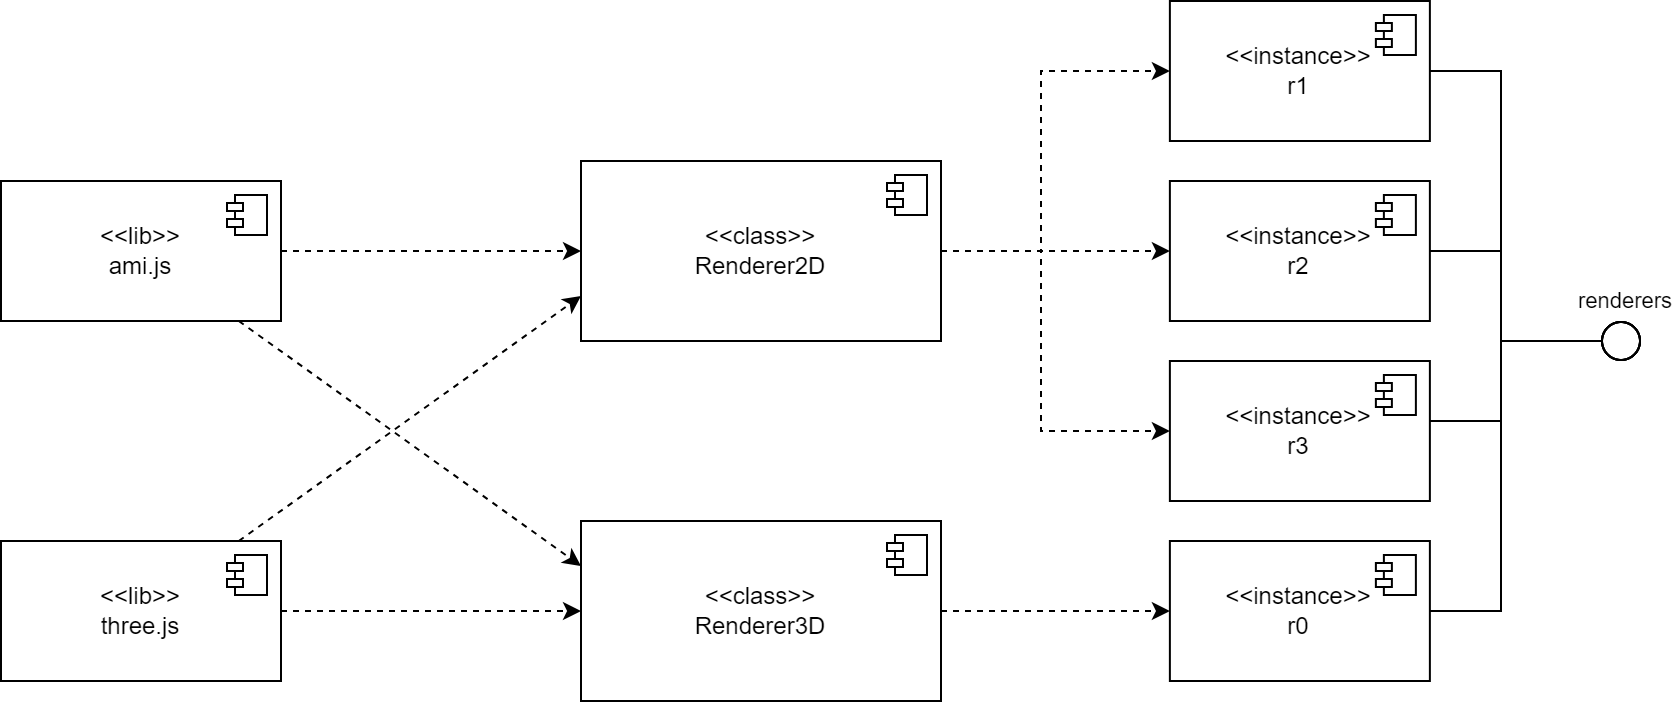
\includegraphics[]{images/chap3/renderers_uml_components.drawio.png}
        \caption{Диаграмма компонентов логики работы с 3D объектами}
        \label{fig:db_scheme}
    \end{figure}

Для удобного доступа к рендерерам в компонентах React были созданы хуки, такие как useRenderer и useRenderers. Эти хуки обеспечивают доступ к рендерерам из любого компонента дерева компонентов, позволяя удобно и эффективно работать с 3D и 2D сценами. Был реализован хук для доступа как ко всем рендерарам, так и к текущему. На \hyperref[fig:hooks]{рисунке \ref*{fig:hooks}} это изображено схематично в диаграмме компонентов.

    \begin{figure}[H]
        \centering
        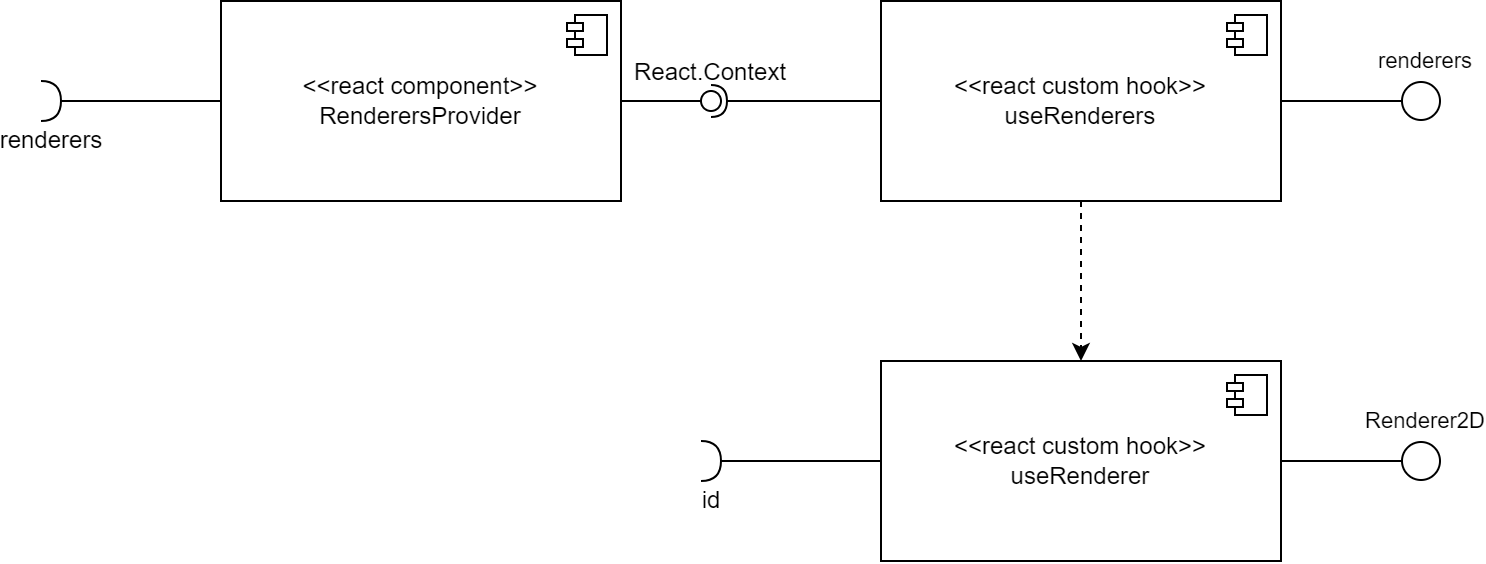
\includegraphics[]{images/chap3/react_uml_components.drawio.png}
        \caption{Диаграмма компонентов доступа рендереров через хуки в UI}
        \label{fig:hooks}
    \end{figure}

\subsection{Компоненты React}

Условно все компоненты можно разделить на три группы:
\begin{itemize}
    \item компоненты, связанные со сценой;
    \item провайдеры;
    \item UI-компоненты.
\end{itemize}

Первые отвечают за инициализацию и управление 3D-сценой, а также за создание и отображение 3D-объектов. Они взаимодействуют с классами Renderer2D и Renderer3D для управления сценами. Список компонентов:
\begin{itemize}
    \item Canvas2D: Компонент для инициализации 2D сцены;
    \item Canvas3D: Компонент для инициализации 3D сцены;
    \item LocalizerHelper: Компонент для работы с локализатором;
    \item StackHelper: Компонент для работы со стеком DICOM;
    \item Aorta: Компонент для отображения сегментированной аорты.
\end{itemize}

Провайдеры обеспечивают управление и доступ к основным элементам системы. Они служат для передачи данных и методов через дерево компонентов, обеспечивая инкапсуляцию и удобное использование ресурсов:
\begin{itemize}
    \item AortaProvider: Обеспечивает доступ к данным сегментированной аорты;
    \item QuadViewProvider: Определяет, какая из сцен используется и управляет четырьмя различными видами;
    \item RenderersProvider: Обеспечивает доступ к классам рендереров для работы с 2D и 3D сценами;
    \item StackProvider: Обеспечивает доступ к DICOM снимкам и управляет их состоянием.
\end{itemize}

UI-компоненты представляют собой элементы пользовательского интерфейса, которые обеспечивают взаимодействие пользователя с системой. Они включают в себя навигационные элементы, списки пациентов и карточки данных пациента:
\begin{itemize}
    \item AppToolbar: Верхняя панель навигации приложения;
    \item AppToolbarButton: Кнопки на верхней панели навигации;
    \item PatientCard: Карточка данных пациента, отображающая информацию о конкретном пациенте;
    \item PatientCardList: Список карточек пациентов, содержащий данные обо всех пациентах;
    \item PatientDataCard: Карточка данных пациента, отображающая информацию о конкретном снимке;
    \item PatientDataCardList: Список карточек данных пациента, содержащий информацию обо всех снимках пациента;
    \item QuadView: Компонент, объединяющий все четыре сцены.
\end{itemize}

\subsection{Взаимодействие с серверной частью}

Общение между клиентом и сервером было реализовано через WebSocket. Для этого было несколько причин:

\begin{itemize}
    \item необходимость отслеживания длительных операций: Процесс выполнения некоторых операций может занимать значительное время. Например, сегментирование аорты выполняется около 30-40 секунд, а моделирование до 3 минут. HTTPS запросы для таких длительных операций неэффективны, так как они не позволяют эффективно отслеживать прогресс и могут приводить к таймаутам. WebSocket позволяет поддерживать постоянное соединение, обеспечивая двустороннюю связь между клиентом и сервером, что позволяет эффективно отслеживать прогресс выполнения операций;
    \item совместимость с Docker-контейнерами: Все решение, включающее все модули, будет упаковано в Docker-контейнер и доступ к серверу и клиенту будет осуществляться с одного и того же домена. Использование HTTPS запросов в данном случае вызывало бы ошибки в браузере из-за политик безопасности, связанных с кросс-доменными запросами. WebSocket позволяет безопасно обходить эти ограничения, обеспечивая надежное взаимодействие между клиентом и сервером;
    \item опыт использования WebSocket в предыдущей версии проекта: взаимодействие с сервером также осуществлялось через WebSocket по аналогичным причинам. Уже была готова некоторая база кода для работы с WebSocket, что облегчило внедрение этой технологии в текущий проект.
\end{itemize}

Было создано API для взаимодействия с сервером, упакованное в отдельный пакет. Это API предоставляет интерфейс для отправки и получения данных через WebSocket. API включает методы для отправки снимков и параметров сегментации (Threshold) на сервер, а также для обработки сообщений, поступающих от сервера. В рамках проекта была проведена работа по реализации типизации для этого API.

Механизм взаимодействия через WebSocket включает следующие шаги:

\begin{enumerate}
    \item Отправка данных на сервер: Клиент отправляет снимки и порог сегментации на сервер через WebSocket.
    \item Обработка сообщений от сервера: Сервер может отправлять сообщения о прогрессе выполнения операции. Когда сервер отправляет сообщение, в API создается искусственное событие.
    \item Подписка на события: на клиенте создается подписка на эти искусственные события с помощью стандартных Event Listener в JavaScript. Например, при получении сообщения о прогрессе сегментации клиент обновляет прогресс бар.
    \item Получение результатов: Когда сервер завершает операцию и отправляет результат (например, STL файл аорты), соответствующее событие срабатывает, и клиент обрабатывает полученные данные.
\end{enumerate}

Схематично взаимодействие сервера и клиента отражено на \hyperref[fig:ws]{рисунке \ref*{fig:ws}}.

\begin{figure}[ht]
    \centering
    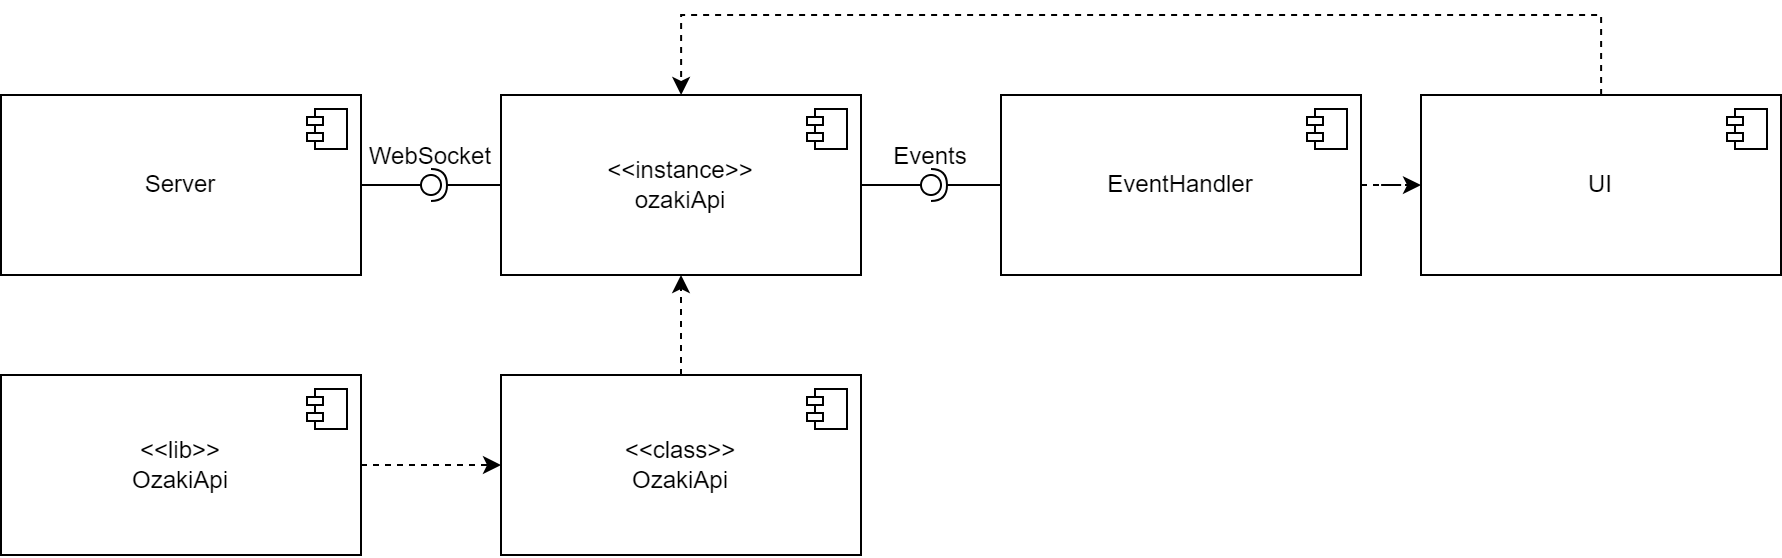
\includegraphics[]{images/chap3/ws_components.drawio.png}
    \caption{Диаграмма компонентов взаимодействия серверной и клиентской части}
    \label{fig:ws}
\end{figure}

STL файл сохраняется в локальную базу данных (Dexie.js) для последующего использования. Для загрузки STL файлов используется модуль Three.js, который обеспечивает визуализацию и дальнейшую работу с 3D моделями.

Таким образом, использование WebSocket для взаимодействия с сервером обеспечило эффективное и надежное выполнение длительных операций, а также позволило реализовать удобный механизм отслеживания прогресса и получения результатов в реальном времени.

Одной из ключевых задач при развертывании клиент-серверного приложения было автоматическое определение URL сервера в production режиме, когда клиент и сервер находятся в одном Docker-контейнере. Для этого была реализована соответствующая функция, которая автоматически определяет URL сервера.

Когда клиентская версия находится в developer режиме, автоматическое определение URL сервера необходимо отключать. В этом режиме удобно вручную вводить нужный URL для тестирования и отладки. Чтобы автоматизировать этот процесс и избежать необходимости ручного переключения URL, использовалась одна из функций сборщика Vite.

Vite позволяет настраивать окружение и переменные окружения, которые фиксируют текущий режим работы (developer или production). В зависимости от режима, в код вставляется соответствующая переменная.

Была настроена система переменных окружения, которая позволяет автоматически переключаться между режимами developer и production. Это существенно упростило процесс разработки и развертывания приложения, так как отпала необходимость вручную править код.

\section{Демонстрация работы приложения}

В этом разделе представлены скриншоты работающего приложения, демонстрирующие основные функции и возможности системы. Визуальные примеры помогают лучше понять, как реализованы и функционируют различные компоненты приложения.

На \hyperref[fig:dicom]{рисунке \ref*{fig:dicom}} показано отображение DICOM снимков на всех четырех сценах. Это позволяет пользователям просматривать снимки пациента в разных проекциях и настраивать параметры визуализации для получения наиболее информативных изображений.

\begin{figure}[h!]
    \centering
    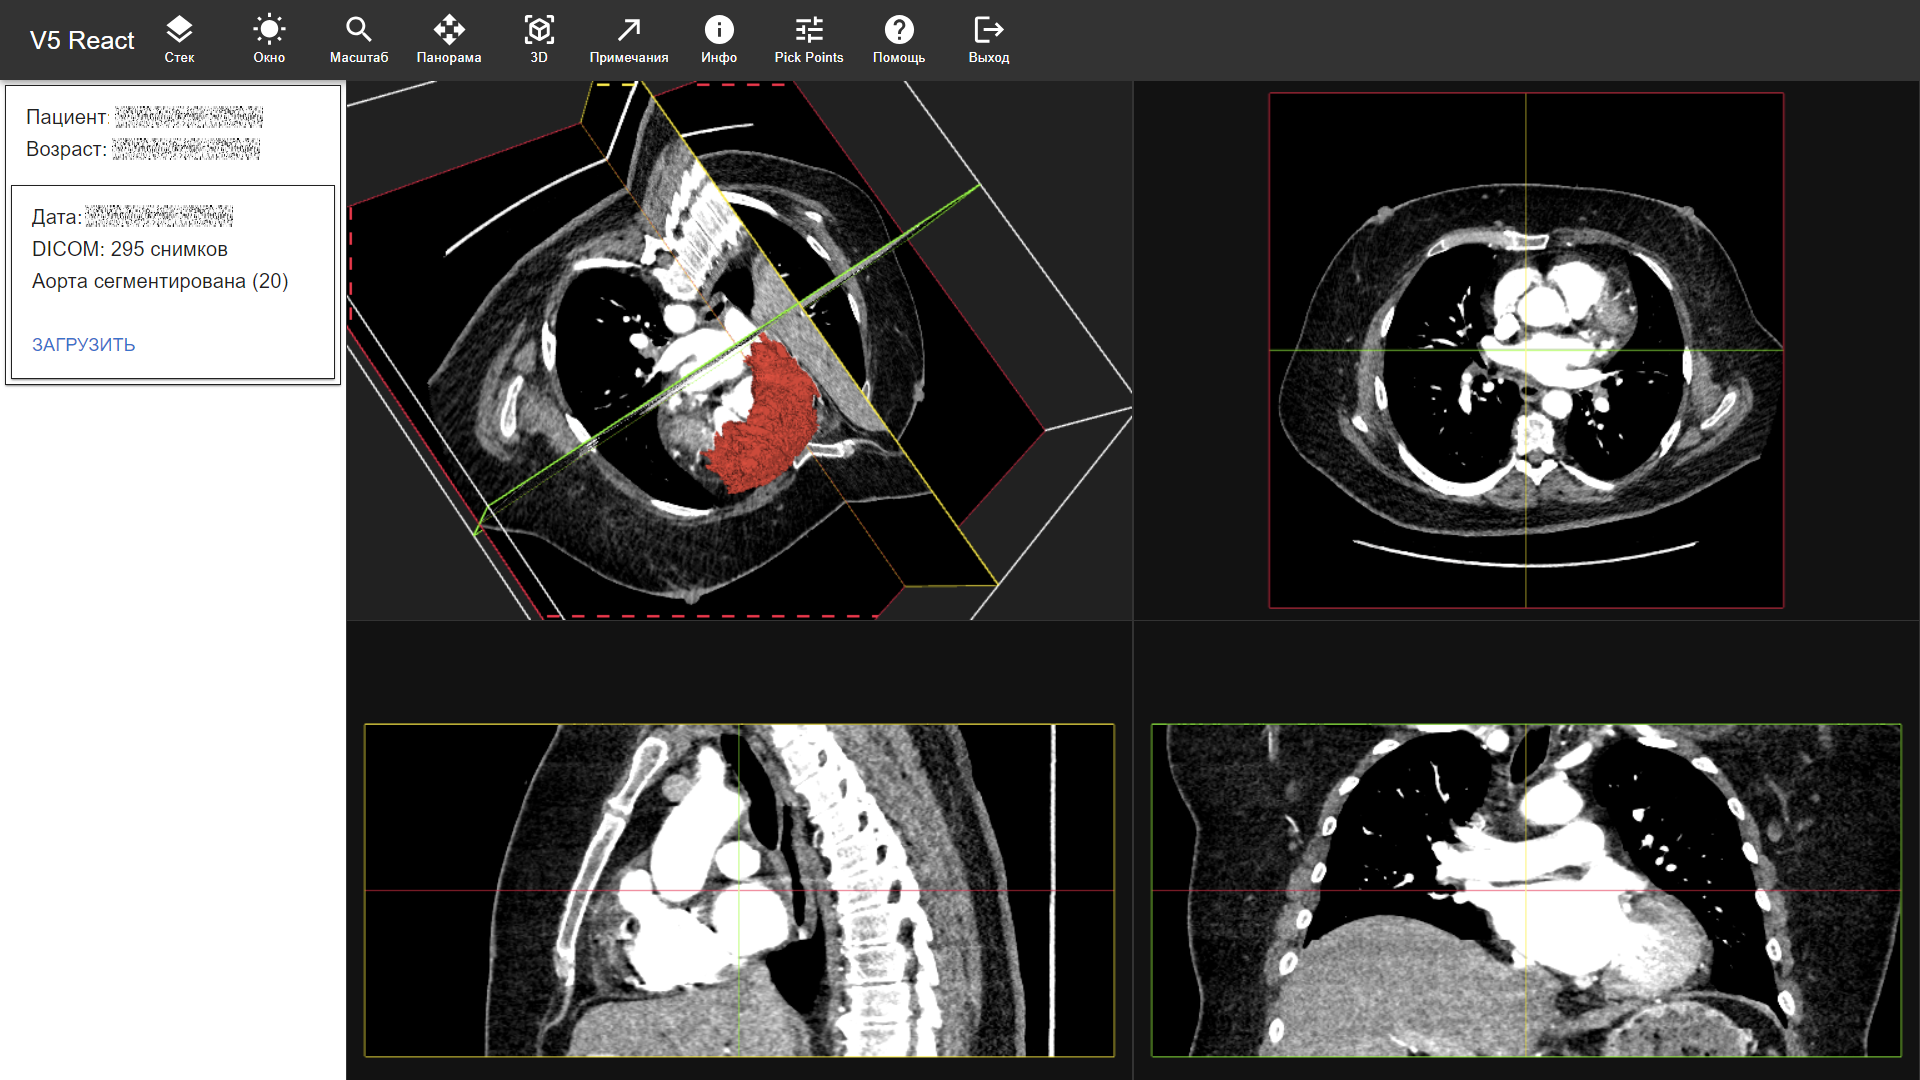
\includegraphics[]{images/chap3/dicom.png}
    \caption{КТ пациента в 3 проекциях}
    \label{fig:dicom}
\end{figure}

На \hyperref[fig:aorta]{рисунке \ref*{fig:aorta}} демонстрируется сегментированная аорта для пациента. Сегментация позволяет выделить аорту на снимках и визуализировать ее в 3D пространстве.

\begin{figure}[H]
    \centering
    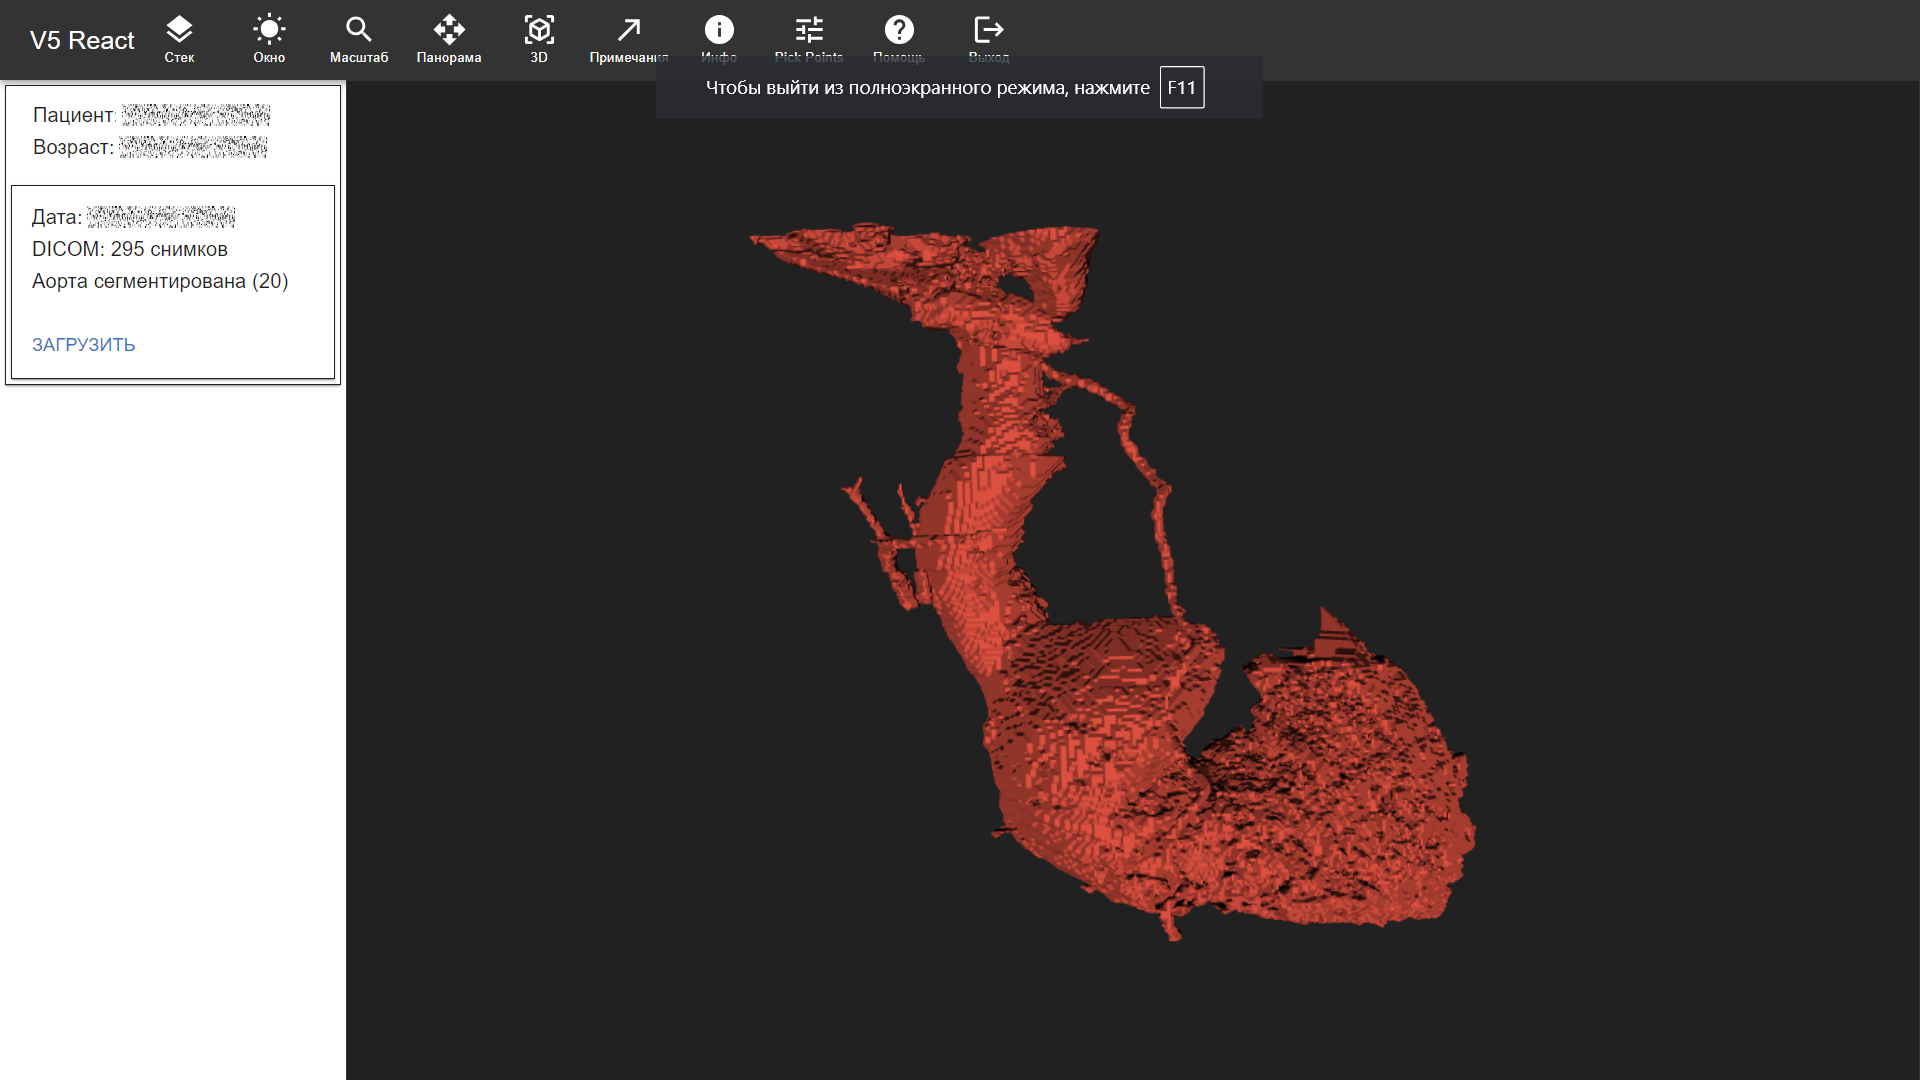
\includegraphics[]{images/chap3/aorta.png}
    \caption{Сегментировная 3D модель аорты}
    \label{fig:aorta}
\end{figure}

На \hyperref[fig:dialog]{рисунке \ref*{fig:dialog}} демонстрируется диалог для сегментации аорты.

\begin{figure}[h!]
    \centering
    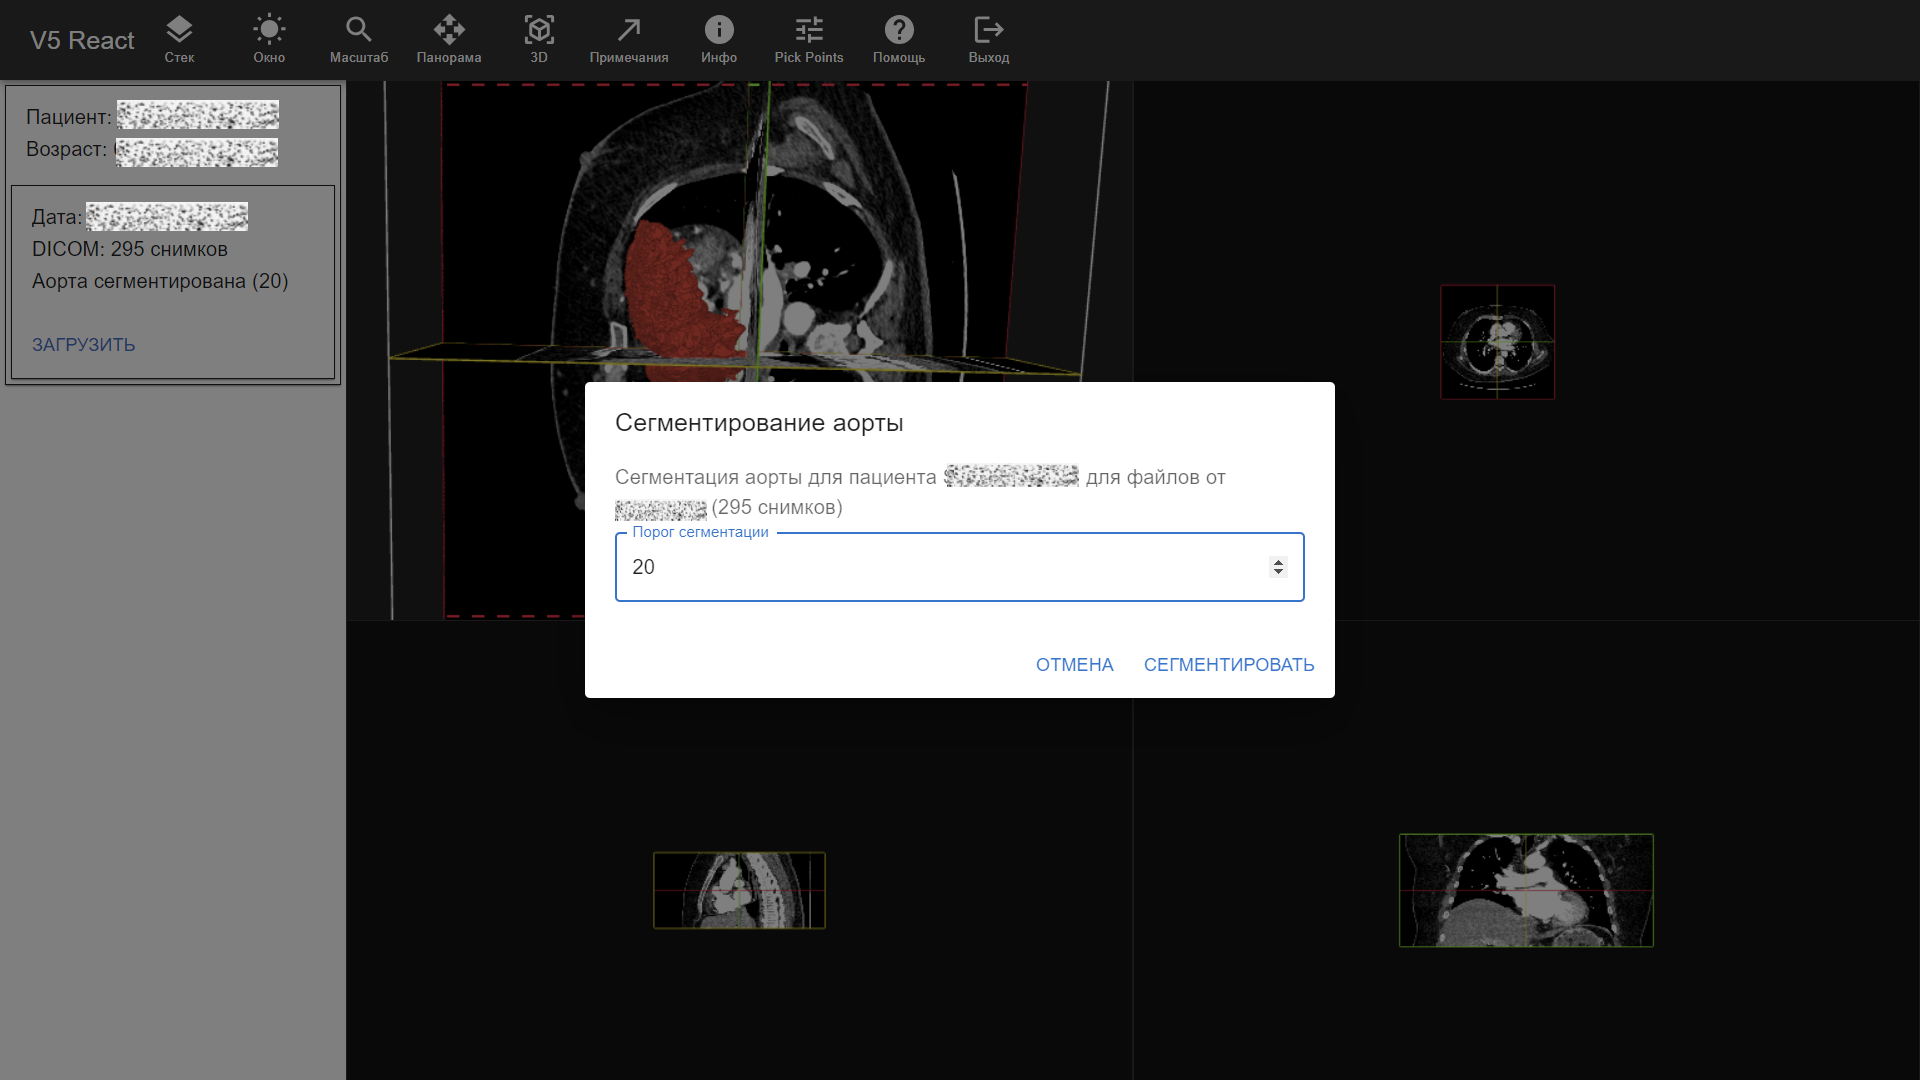
\includegraphics[]{images/chap3/dialog.png}
    \caption{Диалог сегментации аорты}
    \label{fig:dialog}
\end{figure}

На \hyperref[fig:progress]{рисунке \ref*{fig:progress}} демонстрируется отображение прогресса при выполнении сегментации на стороне сервера, что позволяет контролировать и отслеживать выполнение длительных операций.

\begin{figure}[h!]
    \centering
    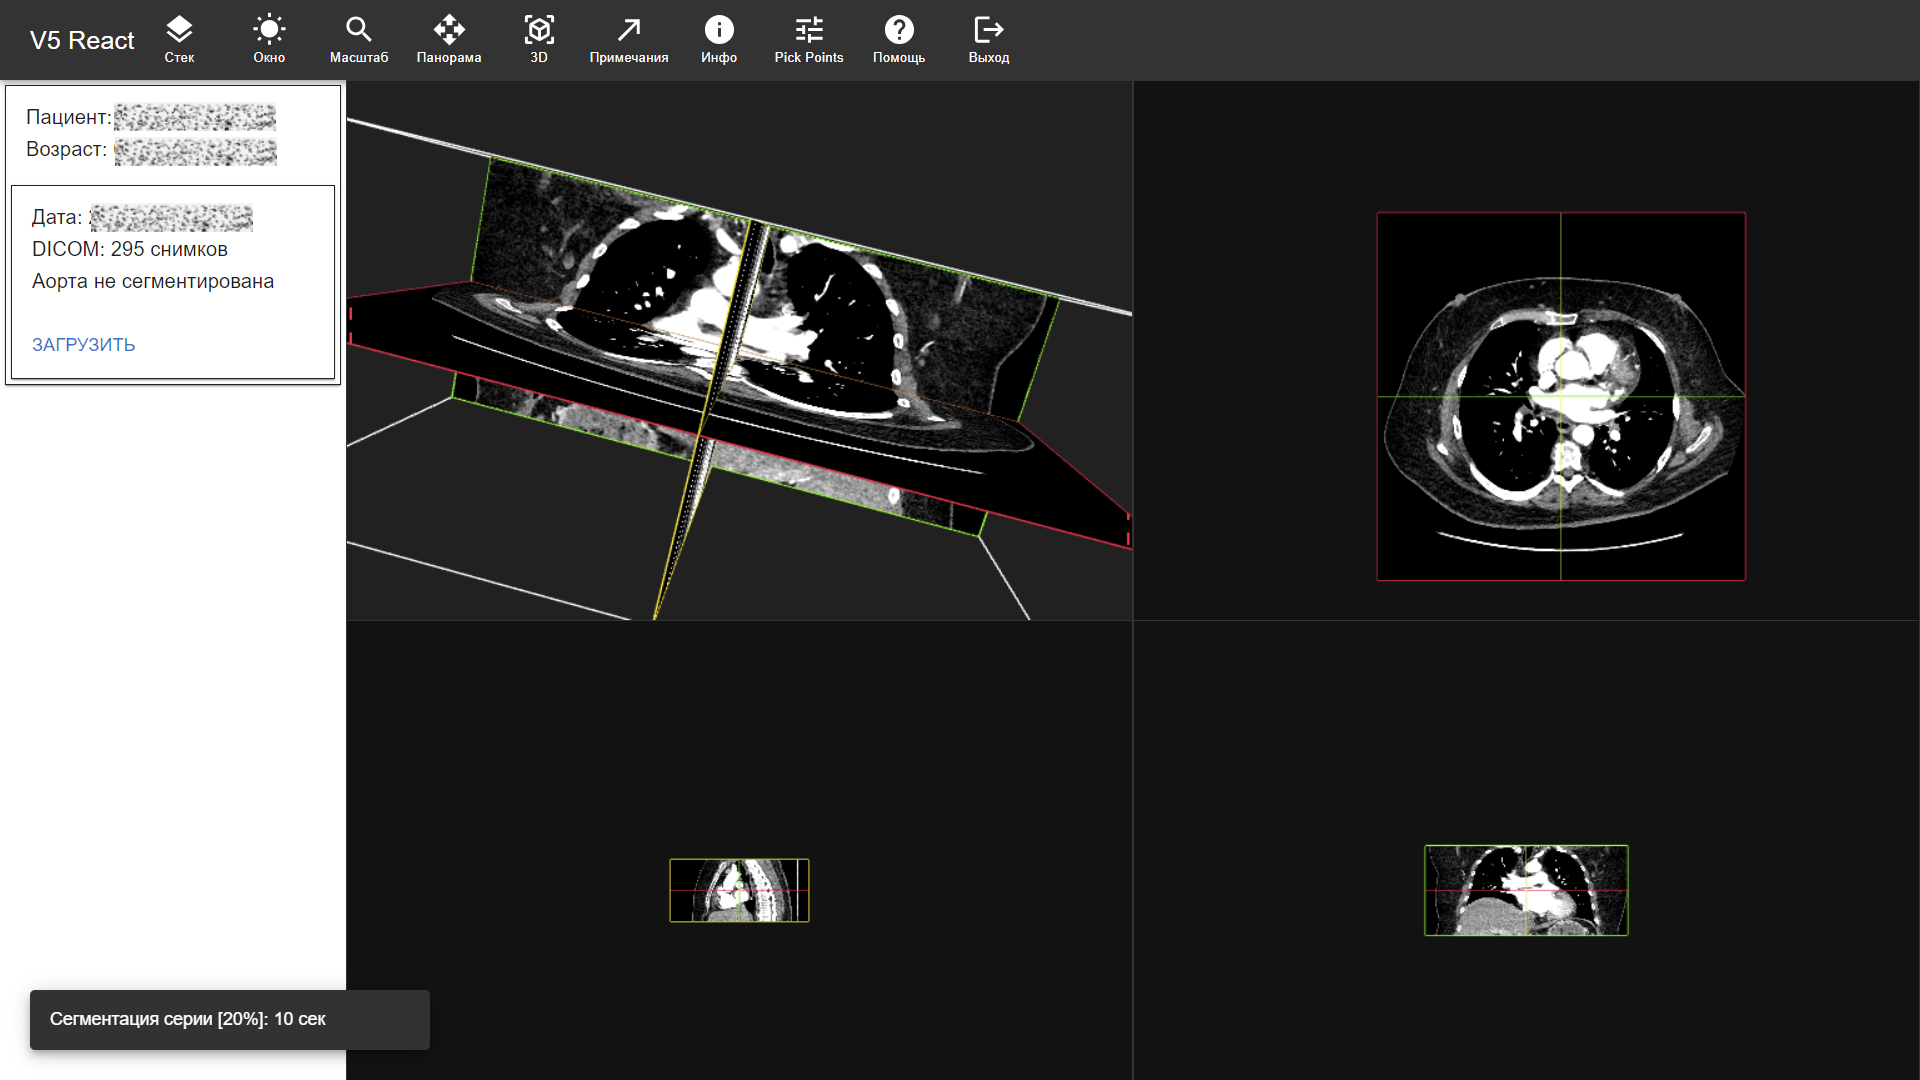
\includegraphics[]{images/chap3/progress.png}
    \caption{Прогресс сегментации}
    \label{fig:progress}
\end{figure}

На данном этапе удалось реализовать только две из четырех основных функций, описанных в разделе \hyperref[subsec:req]{разделе \ref{subsec:req}}. В частности, были разработаны интерфейсы для загрузки данных пациента и их просмотра, а также сегментация и визуализация аорты.

Разработка следующих функций, таких как проведение линий пришивания створок клапана аорты и визуализация результатов моделирования, будет следующим шагом в развитии проекта. Эти функции планируется реализовать в рамках последующих этапов работы.

\endinput